\begin{savequote}[45mm]
\ascii{Any fool can write code that a computer can understand. Good programmers write code that humans can understand.}
\qauthor{\ascii{- Martin Flower}}
\end{savequote}

\chapter{再解耦合} 
\label{ch:redecoupling}

\begin{content}

\end{content}

\section{耦合1}

\begin{content}

\subsection{坏味道}

观察\code{TestCase::run}的逻辑实现,其实现逻辑与\ascii{TestResult}关系更加密切。因为,\code{TestCase::run}的每个语句都是通过调用\ascii{TestResult}成员函数完成的。其中,宏函数\ascii{PROTECT}也是通过调用\ascii{TestResult::protect}成员函数完成的,只是宏实现掩盖了这个隐式关系。

\begin{nodiff}{include/mars/core/TestCase.cc}
 \begin{c++}
#include <mars/core/TestCase.h>
#include <mars/core/TestResult.h>
#include <mars/core/internal/TestCaseFunctor.h>

// ...

#define PROTECT(method) \
  result.protect(Functor(this, &TestCase::method,  "in the "#method))

void TestCase::runBare(TestResult& result) {
  if (PROTECT(setUp)) {
    PROTECT(runTest);
  }
  PROTECT(tearDown);
}

void TestCase::run(TestResult& result) {
  result.startTestCase(*this);
  runBare(result);
  result.endTestCase(*this);
}
 \end{c++}
\end{nodiff}

由于\ascii{TestCase}与\ascii{TestResult}之间职责分配不合理,导致\ascii{TestResult}不得不公开\ascii{startTestCase, endTestCase, protect}三个成员函数,急剧增强了\ascii{TestCase::run}对\ascii{TestResult}的依赖关系。

\begin{nodiff}{include/mars/core/TestResult.h}
 \begin{c++}
struct Test;
struct TestCaseFunctor;

struct TestResult {
  // ...

  void startTestCase(const Test&);
  void endTestCase(const Test&);

  bool protect(const TestCaseFunctor&);
};
 \end{c++}
\end{nodiff}

\subsubsection{友元关系}

可以声明\ascii{TestCase}为\ascii{TestResult}的友元类,从而实现\ascii{startTestCase, endTestCase, protect}的私有化。但是,友元声明将导致\ascii{TestResult}完全地失去了信息隐藏的保护机制,严重地破坏了\ascii{TestResult}的封装特性。

关键在于,使用友元并没有降低\ascii{TestCase::run}对\ascii{TestResult}的依赖强度,甚至加剧了两者之间的耦合关系。毕竟\ascii{TestResult}已经为\ascii{TestCase}敞开门户,任由\ascii{TestCase}在其领地无限制地驰骋,毫无隐私可言。一般地,在\ascii{99.99\%}的场景下,都需要拒绝友元的诱惑。

\begin{nodiff}{include/mars/core/TestResult.h}
 \begin{c++}
struct Test;
struct TestCaseFunctor;

struct TestResult {
  // ...

private:
  void startTestCase(const Test&);
  void endTestCase(const Test&);
  bool protect(const TestCaseFunctor&);

  friend struct TestCase;
};
 \end{c++}
\end{nodiff}

\subsection{试错}

根据\emph{迪米特法则},与其让\ascii{TestCase::run}详尽地告诉\ascii{TestResult}按部就班地调用\ascii{startTestCase, endTestCase, protect}三个成员函数完成实现逻辑,不如直接让\ascii{TestResult}自己将这三个成员函数封装起来,仅提供唯一公开的接口\ascii{TestResult::runTestCase}给\ascii{TestCase}访问即可。一方面,缩小了\ascii{TestCase}对\ascii{TestResult}的依赖范围。另一方面,使得\ascii{TestResult}得到更好的封装特性。

\subsubsection{搬迁职责: 从TestCase至TestResult}

首先,在\ascii{TestResult}头文件中,将既有的成员函数\ascii{startTestCase, endTestCase, protect}私有化,仅对外提供唯一的公开接口\ascii{runTestCase}给\ascii{TestCase}访问。

\begin{nodiff}{include/mars/core/TestResult.h}
 \begin{c++}
struct Test;
struct TestCase;
struct TestCaseFunctor;

struct TestResult {
  // ...

  void runTestCase(TestCase&);

private:
  void startTestCase(const Test&);
  void endTestCase(const Test&);
  bool protect(const TestCaseFunctor&);
};
 \end{c++}
\end{nodiff}

在\ascii{TestResult}实现文件中,将\ascii{TestCase::run}的逻辑搬迁至\ascii{TestResult::runTestCase}。同理,将\ascii{TestCase.cc}既有实现的\ascii{runBare, Functor, PROTECT}一并搬迁至\ascii{TestResult.cc},少许修改宏定义\ascii{PROTECT}即可工作。

\begin{nodiff}{src/mars/core/TestResult.cc}
 \begin{c++}
#include <mars/core/TestResult.h>
#include <mars/core/TestListener.h>
#include <mars/core/internal/TestCaseFunctor.h>
#include <mars/core/TestCase.h>

namespace {
  struct Functor : TestCaseFunctor {
    using Method = void(TestCase::*)();

    Functor(TestCase& self, Method method, const char* place)
      : self(self), method(method), place(place) {
    }

  private:
    const char* where() const override {
      return place;
    }

    bool operator()() const override {
      (self->*method)();
      return true;
    }

  private:
    TestCase* self;
    Method method;
    const char* place;
  };
}

#define PROTECT(method) \
  protect(Functor(&test, &TestCase::method,  "in the "#method))

void TestResult::runBare(TestCase& test) {
  if (PROTECT(setUp)) {
    PROTECT(runTest);
  }
  PROTECT(tearDown);
}

#define BOARDCAST(action) \
  for (auto listener : listeners) listener->action

void TestResult::runTestCase(TestCase& test) {
  BOARDCAST(startTestCase(test));
  runBare(test);
  BOARDCAST(startTestCase(test));
}

// ...
 \end{c++}
\end{nodiff}

从最终搬迁效果看,已经删除\ascii{TestResult}中既有的成员函数\ascii{startTestCase, endTestCase},而不仅仅只是私有化,毕竟它们都仅仅包含一行有效语句,完全可以内联化,将其干掉。待搬迁完成后,\ascii{TestCase::run}通过调用\ascii{TestResult::runTestCase}启动执行。

\begin{nodiff}{src/mars/core/TestCase.cc}
 \begin{c++}
void TestCase::run(TestResult& result) {
  result.runTestCase(*this);
}
 \end{c++}
\end{nodiff}

但是,此时\ascii{TestResult.cc}编译失败。编译期要求\ascii{TestCase}公开\ascii{setUp, tearDown, runTest}三个成员函数。为了修正这个编译问题,\ascii{TestFixture}的私有继承重构为共有继承,\ascii{TestCase::runTest}子函数实现也搬迁至公开域。

\begin{nodiff}{include/mars/core/TestCase.h}
 \begin{c++}
#include <mars/core/Test.h>
#include <mars/core/TestFixture.h>

struct TestCase : Test, TestFixture {
  using Test::Test;

  virtual void runTest() {}

private:
  void run(TestResult&) override;
  int countTestCases() const override;
};
 \end{c++}
\end{nodiff}

重构完毕,测试通过。不幸的是,熊掌与鱼翅不可兼得,收获了\ascii{TestResult}的封装性,但牺牲了\ascii{TestCase}的封装性。

\subsubsection{搬迁职责: 从TestResult至TestCase}

仔细观察\ascii{TestCase::runBare}的原始实现,很难辨别其到底是与\ascii{TestCase}关系亲密,还是与\ascii{TestResult}关系更亲密。

在之前的重构基础智商,再将\ascii{Functor, PROTECT, runBare}搬迁回\ascii{TestCase.cc}之中,则必然要求\ascii{TestResult}公开\ascii{protect}成员函数。此时,相对原始的\ascii{TestCase}与\ascii{TestResult}实现,设计改进甚微,得不偿失。

经过两轮重构尝试,事实证明是失败的。无论\ascii{TestCase::runBare}在那一方实现,都要破坏另一方的封装性;\ascii{TestCase}与\ascii{TestResult}之间是相互依赖的,不仅仅只是\ascii{TestCase}单方面依赖于\ascii{TestResult}。使用\ascii{Git}回到原始状态,尝试新的重构思路。

\begin{nodiff}{重构失败,回滚修改}
 \begin{c++}
$ git reset --hard master
 \end{c++}
\end{nodiff}

\subsubsection{理想情况}

在最理想的情况下,一方面,\ascii{TestResult}仅向\ascii{TestCase}提供唯一的公开接口\ascii{runTestCase},而私有化成员函数\ascii{protect},内联化成员函数\ascii{startTestCase, endTestCase}。另一方面,还要保持\ascii{TestCase}既有的封装性,包括私有继承\ascii{TestFixture},及其私有化成员函数\ascii{runTest, runBare}。

在之前两轮重构失败的经验之上,让我们找到了潜在的抽象。借助于抽象的隔离,最小化\ascii{TestCase}与\ascii{TestResult}之间的依赖关系,最终使得\ascii{TestCase}唯一地依赖于\ascii{TestResult::runTestCase}接口。一方面,满足迪米特法则的基本原则,使得\ascii{TestResult}获得更好的封装性。另一方面,极大地缩小了\ascii{TestCase}与\ascii{TestResult}的依赖范围,符合正交设计的基本原则。

\subsection{关键抽象}

在新的一轮重构中,将在\ascii{TestCase.cc}中保留\ascii{runBare, Functor, PROTECT}的所有实现,仅将\ascii{TestCase::run}的逻辑搬迁至\ascii{TestResult::runTestCase}之中。为了保证\ascii{TestCase::runBare}看不到\ascii{TestResult::protect}成员函数,在它们两者之间建立抽象\ascii{TestCaseProtector},解除这两个成员函数之间的耦合关系。

\begin{nodiff}{include/mars/core/internal/TestCaseProtector.h}
 \begin{c++}
struct TestCaseFunctor;

struct TestCaseProtector {
  virtual bool protect(const TestCaseFunctor&) = 0;
  virtual ~TestCaseProtector() {}
};
 \end{c++}
\end{nodiff}

同时,为了保证\ascii{TestResult::runTestCase}看不到\ascii{TestCase::runBare},在两者之间建立抽象\ascii{BareTestCase},解除这两个成员函数之间的耦合关系。

\begin{nodiff}{include/mars/core/internal/BareTestCase.h}
 \begin{c++}
struct Test;
struct TestCaseProtector;

struct BareTestCase {
  virtual const Test& get() const = 0;
  virtual void runBare(TestCaseProtector&) = 0;

  virtual ~BareTestCase() {}
};
 \end{c++}
\end{nodiff}

\subsubsection{私有继承: BareTestCase}

\ascii{TestCase}私有继承自\ascii{BareTestCase},当覆写成员函数\ascii{runBare, get}时,保证对外不可见,使其具有更好的封装特性。

\begin{nodiff}{include/mars/core/TestCase.h}
 \begin{c++}
#include <mars/core/Test.h>
#include <mars/core/TestFixture.h>
#include <mars/core/internal/BareTestCase.h>

struct TestCase
  : Test
  , private TestFixture
  , private BareTestCase {

  using Test::Test;

private:
  void run(TestResult&) override;
  int countTestCases() const override;

private:
  const Test& get() const override;
  void runBare(TestCaseProtector&) override;

private:
  virtual void runTest() {}
};
 \end{c++}
\end{nodiff}

在实现文件中,\ascii{TestCase::runBare}不再依赖于具体的\ascii{TestResult}类型,而是依赖于抽象的\ascii{TestCaseProtector},从而解除了\ascii{TestCase::runBare}对\ascii{TestResult}的依赖关系。

为了遵循迪米特法则,重构\ascii{TestCase::run}的实现逻辑,使其调用公开给\ascii{TestCase}的唯一接口\ascii{TestResult::runTestCase},实现了\ascii{TestResult}内部中封装广播事件等实现细节。

最为关键的是,在\ascii{TestCase::run}实现中,传递\ascii{this}所指的当前对象至\ascii{TestResult::runTest\\-Case(BareTestCase\&)}成员函数。因为\ascii{TestCase}私有继承自\ascii{BareTestCase},在\ascii{TestCase}类域中,\ascii{this}所指的当前对象是\ascii{BareTestCase}合法的\emph{私生子}。

\begin{nodiff}{include/mars/core/TestCase.cc}
 \begin{c++}
#include <mars/core/TestCase.h>
#include <mars/core/TestResult.h>
#include <mars/core/internal/TestCaseProtector.h>

// ...

#define PROTECT(method) \
  p.protect(Functor(this, &TestCase::method,  "in the "#method))

void TestCase::runBare(TestCaseProtector& p) {
  if (PROTECT(setUp)) {
    PROTECT(runTest);
  }
  PROTECT(tearDown);
}

const Test& TestCase::get() const {
  return *this;
}

void TestCase::run(TestResult& result) {
  result.runTestCase(*this);
}
 \end{c++}
\end{nodiff}

\subsubsection{私有继承: TestCaseProtector}

\ascii{TestResult}私有继承自\ascii{TestCaseProtector}。当覆写成员函数\ascii{protect},保证不对外公开,使其具有更好的封装特性。

\begin{nodiff}{include/mars/core/TestResult.h}
 \begin{c++}
#include <vector>
#include <mars/core/internal/TestCaseProtector.h>

struct TestListener;
struct BareTestCase;

struct TestResult : private TestCaseProtector {
  // ...
  void runTestCase(BareTestCase&);

private:
  bool protect(const TestCaseFunctor&) override;

private:
  std::vector<TestListener*> listeners;
};
 \end{c++}
\end{nodiff}

在\ascii{TestResult::runTestCase}实现中,已经内联化既有的成员函数\ascii{startTestCase, endTestCase}。最为关键的是,在\ascii{TestResult::runTestCase}实现中,传递\code{this}所指的当前对象至成员函数\ascii{BareTestCase::runBare(TestCaseProtector\&)}。因为\ascii{TestResult}私有继承自\ascii{TestCaseProtector},在\ascii{TestResult}类域中,\code{this}所指的当前对象是\ascii{TestCaseProtector}合法的\emph{私生子}。

\begin{nodiff}{src/mars/core/TestResult.cc}
 \begin{c++}
#include <mars/core/TestResult.h>
#include <mars/core/TestListener.h>
#include <mars/core/internal/BareTestCase.h>

// ...

#define BOARDCAST(action) \
  for (auto listener : listeners) listener->action

void TestResult::runTestCase(BareTestCase& test) {
  BOARDCAST(startTestCase(test.get()));
  test.runBare(*this);
  BOARDCAST(endTestCase(test.get()));
}
 \end{c++}
\end{nodiff}

\subsection{重构回顾}

在重构之前,\ascii{TestCase::run}需要在\ascii{TestCase::runBare}前后分别调用公开的\ascii{TestResult::startTestCase, TestResult::endTestCase},导致\ascii{TestCase::run}的实现逻辑,严重依赖于\ascii{TestResult}广播事件的具体实现细节。

\begin{figure}[H]
\centering
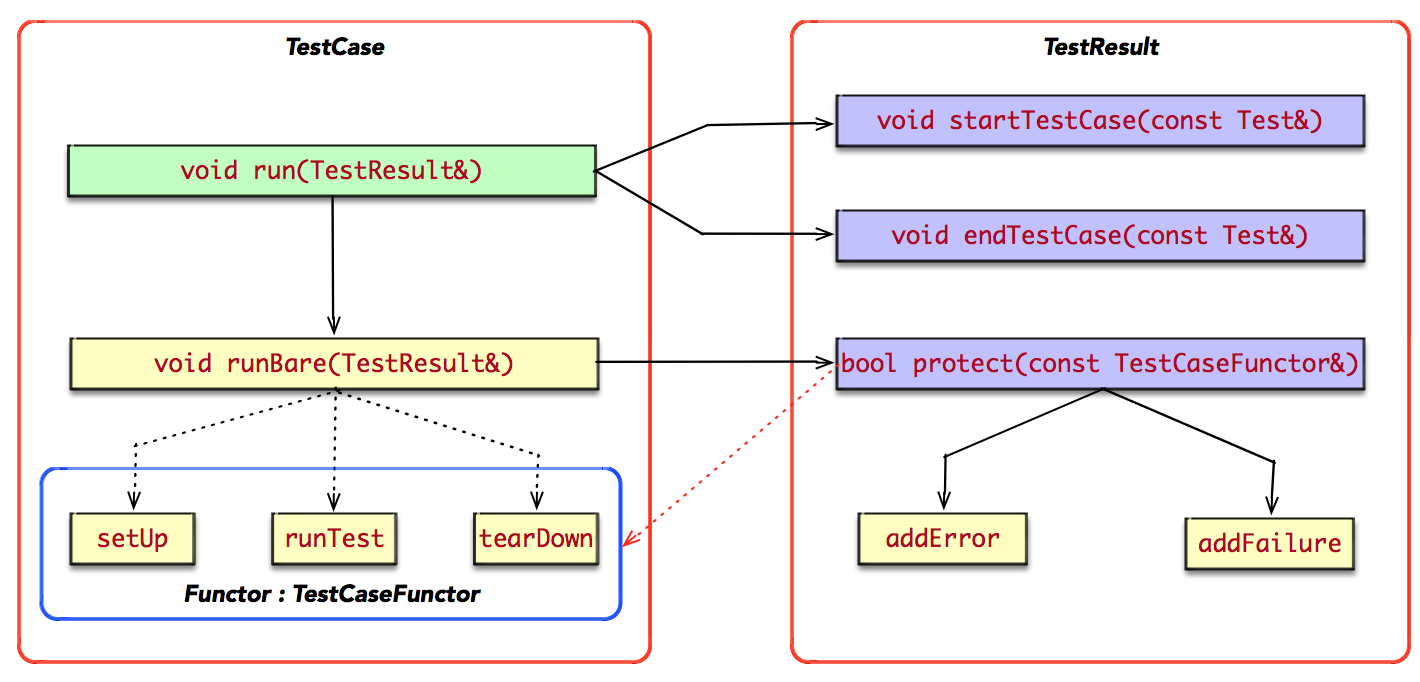
\includegraphics[width=1.0\textwidth]{figures/xunit/decoupling-1-1.png}
\caption{重构之前}
 \label{fig:decoupling-1-1-2}
\end{figure}

根据迪米特法则,将\ascii{TestCase::run}搬迁至\ascii{TestResult::runTestCase}。一方面,\ascii{TestResult}暴露给\ascii{TestCase}接口由\ascii{2}减少至\ascii{1},缓解了\ascii{TestCase}对\ascii{TestResult}的依赖关系。另一方面,实现\ascii{TestResult::startTestCase, TestResult::endTestCase}的私有化或内联化,使得\ascii{TestResult}获得了更好的封装特性。

\begin{figure}[H]
\centering
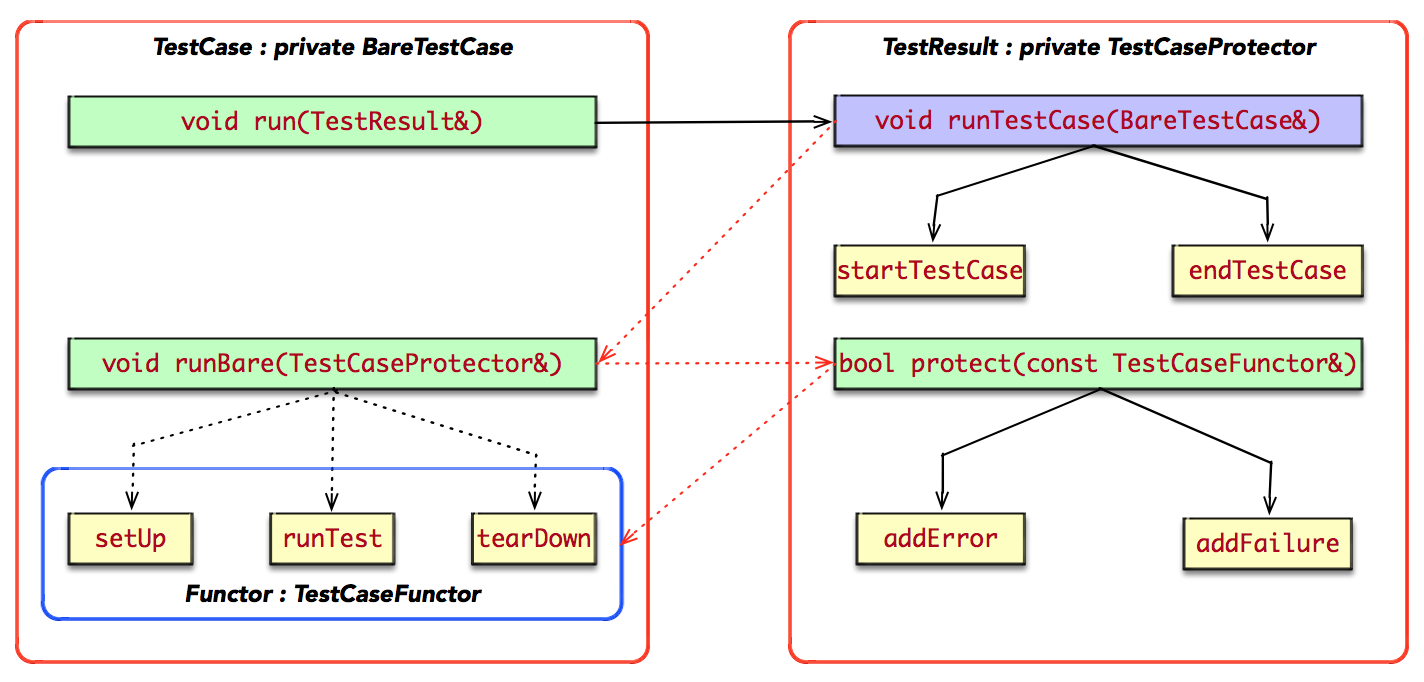
\includegraphics[width=1.0\textwidth]{figures/xunit/decoupling-1-2.png}
\caption{重构之后}
 \label{fig:decoupling-1-2}
\end{figure}

解耦的关键在于抽象接口\ascii{BareTestCase}和\ascii{TestCaseProtector}。前者使得\ascii{TestResult::runTestCase}不再依赖于具体的\ascii{TestCase},使得\ascii{TestCase::runBare}获得了良好的封装性。后者使得\ascii{TestCase::runBare}不再依赖于具体的\ascii{TestResult},使得\ascii{TestResult::protect}获得了良好的封装性。

\begin{figure}[H]
\centering
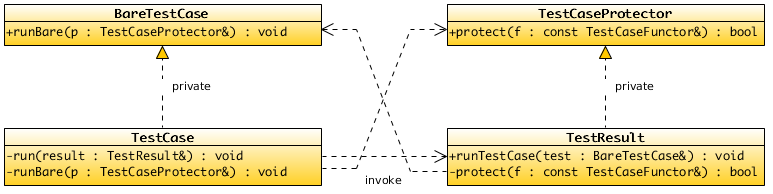
\includegraphics[width=1.0\textwidth]{figures/xunit/bare-test-case-uml.png}
\caption{关键抽象: BareTestCase与TestCaseProtector}
 \label{fig:bare-test-case-uml}
\end{figure}

\end{content}

\section{耦合2}

\begin{content}

\subsection{坏味道}

观察\ascii{TestSuite::run}的实现逻辑,其实现逻辑与\ascii{TestResult}关系更加密切。因为,\code{TestSuite::run}调用\code{TestSuite::runBare}前后两个语句都是调用\ascii{TestResult}的成员函数完成的。与之相反,\ascii{TestSuite::runBare}与\ascii{TestSuite}更加紧密,因为它需要遍历私有数据成员\ascii{tests}\footnote{间接通过成员函数\ascii{foreach}完成。}。

\begin{nodiff}{include/mars/core/TestSuite.cc}
 \begin{c++}
#include <mars/core/TestSuite.h>
#include <mars/core/TestResult.h>

// ...

void TestSuite::runBare(TestResult& result) {
  foreach([&result](auto test) {
    test->run(result);
  });
}

void TestSuite::run(TestResult& result) {
  result.startTestSuite(*this);
  runBare(result);
  result.endTestSuite(*this);
}
 \end{c++}
\end{nodiff}

\subsection{关键抽象}

按照迪米特法则,搬迁\ascii{TestSuite::run}的实现逻辑至\ascii{TestResult::runTestSuite}之中。为了保证\ascii{TestResult::runTestSuite}看不到\ascii{TestSuite::runBare},在两者之间建立抽象\ascii{BareTestSuite},解除这两个成员函数之间的耦合关系。

\begin{nodiff}{include/mars/core/internal/BareTestSuite.h}
 \begin{c++}
struct Test;
struct TestResult;

struct BareTestSuite {
  virtual const Test& get() const = 0;
  virtual void runBare(TestResult&) = 0;

  virtual ~BareTestSuite() {}
};
 \end{c++}
\end{nodiff}

\subsubsection{私有继承: BareTestSuite}

\ascii{TestSuite}私有继承自\ascii{BareTestSuite}。当覆写成员函数\ascii{runBare, get}时,保证对外不公开,使其具有更好的封装特性。

\begin{nodiff}{include/mars/core/TestCase.h}
 \begin{c++}
#include <vector>
#include <mars/core/Test.h>
#include <mars/core/internal/BareTestSuite.h>

struct TestResult;

struct TestSuite : Test, private BareTestSuite {
  // ...

private:
  void run(TestResult& result) override;
  int countTestCases() const override;

private:
  const Test& get() const override;
  void runBare(TestResult& result) override;

private:
  std::vector<Test*> tests;
};
 \end{c++}
\end{nodiff}

在\ascii{TestSuite::run}实现中,传递\ascii{this}所指的当前对象至\ascii{TestResult::runTestSuite(BareTest\\-Suite\&)}。因为\ascii{TestSuite}私有继承自\ascii{BareTestSuite},在\ascii{TestSuite}类域中,\code{this}所指的当前对象是\ascii{BareTestSuite}合法的\emph{私生子}。

\begin{nodiff}{include/mars/core/TestSuite.cc}
 \begin{c++}
#include <mars/core/TestSuite.h>
#include <mars/core/TestResult.h>

// ...

void TestSuite::runBare(TestResult& result) {
  foreach([&result](auto test) {
    test->run(result);
  });
}

const Test& TestSuite::get() const {
  return *this;
}

void TestSuite::run(TestResult& result) {
  result.runTestSuite(*this);
}
 \end{c++}
\end{nodiff}

\subsubsection{搬迁职责}

为了遵循迪米特法则的基本原则,搬迁\ascii{TestSuite::run}的实现逻辑至\ascii{TestResult::runTestSuite}之中,并内联化既有的成员函数\ascii{startTestSuite, endTestSuite}。

因为\ascii{TestResult::runTestSuite}不再依赖与具体的\ascii{TestSuite},而是依赖于更为抽象的\ascii{BareTestSuite}类型,解除了\ascii{TestResult::runTestSuite}对\ascii{TestSuite}的依赖关系。

\begin{nodiff}{include/mars/core/TestResult.cc}
 \begin{c++}
#include <mars/core/TestResult.h>
#include <mars/core/TestListener.h>
#include <mars/core/internal/BareTestSuite.h>

// ...

#define BOARDCAST(action) \
  for (auto listener : listeners) listener->action

void TestResult::runTestSuite(BareTestSuite& test) {
  BOARDCAST(startTestSuite(test.get()));
  test.runBare(*this);
  BOARDCAST(endTestSuite(test.get()));
}
 \end{c++}
\end{nodiff}

\subsection{重构回顾}

在重构之前,在\ascii{TestSuite::run}在\ascii{TestSuite::runBare}的前后分别调用公开的\ascii{TestResult::startTestSuite, TestResult::endTestSuite}。导致\ascii{TestSuite::run}的实现逻辑,严重依赖于\ascii{TestResult}广播事件的具体实现。

\begin{figure}[H]
\centering
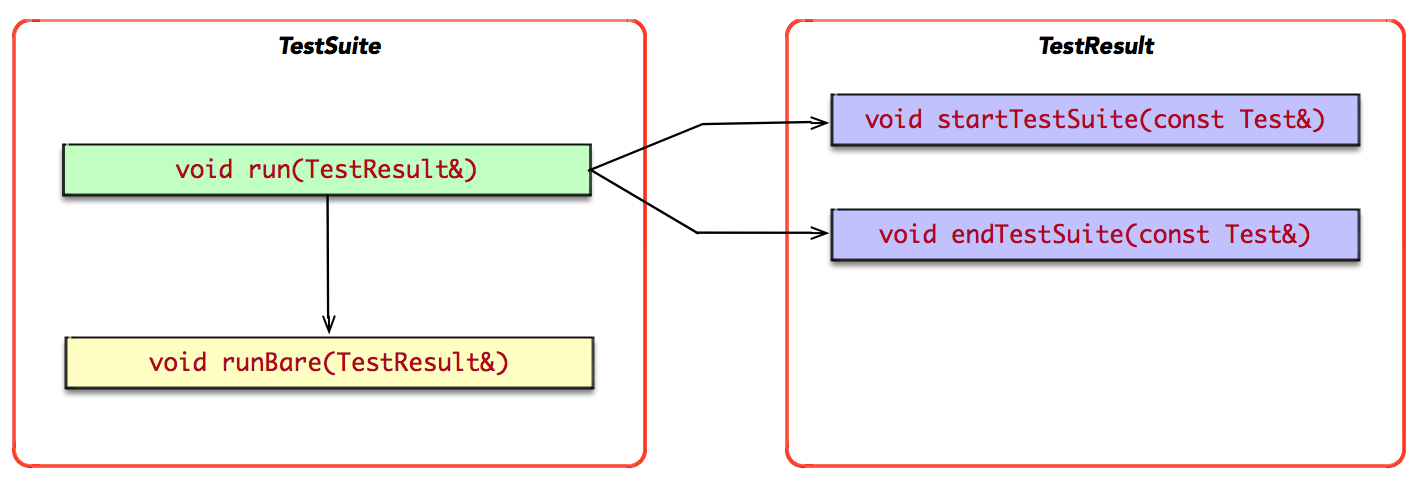
\includegraphics[width=1.0\textwidth]{figures/xunit/coupling-2.png}
\caption{重构之前}
 \label{fig:coupling-2}
\end{figure}

根据迪米特法则,将\ascii{TestSuite::run}搬迁至\ascii{TestResult::runTestSuite}。一方面,\ascii{TestResult}暴露给\ascii{TestCase}接口由\ascii{2}减少至\ascii{1},缓解了\ascii{TestCase}对\ascii{TestResult}的依赖关系。另一方面,内联化\ascii{TestResult::startTestSuite, TestResult::endTestSuite},使得\ascii{TestResult}取得了更好的封装特性。

\begin{figure}[H]
\centering
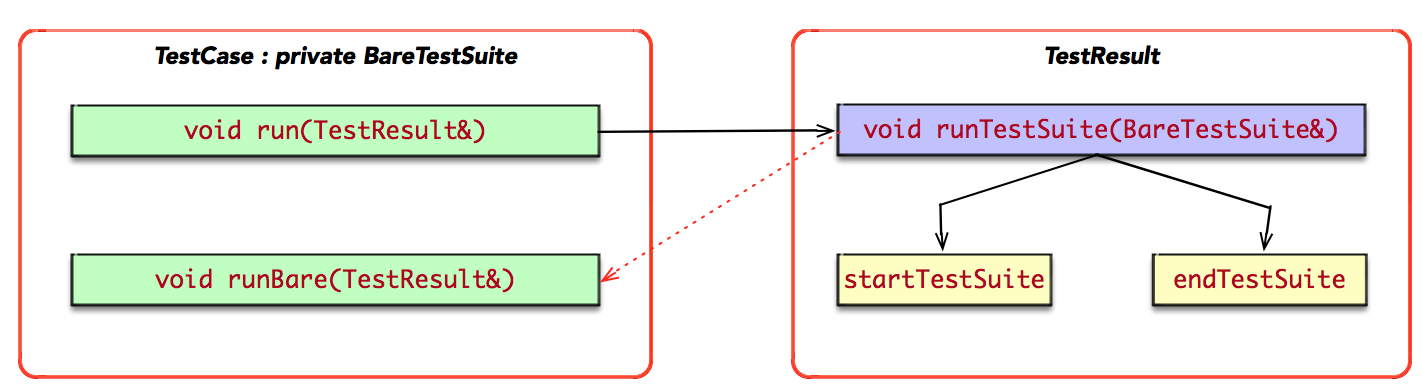
\includegraphics[width=1.0\textwidth]{figures/xunit/decoupling-2.png}
\caption{重构之后}
 \label{fig:decoupling-2}
\end{figure}

解耦的关键在于抽象接口\ascii{BareTestSuite}。在没有破坏\ascii{TestSuite}既有封装特性的前提下,使得\ascii{TestResult::runTestSuite}不再依赖于具体的\ascii{TestSuite}。

\begin{figure}[H]
\centering
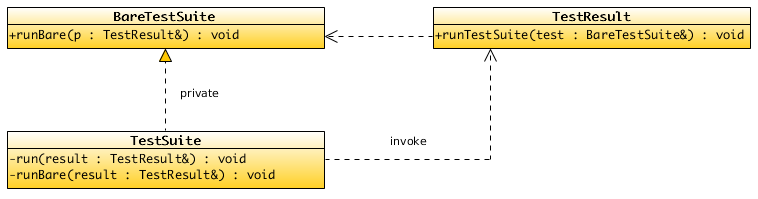
\includegraphics[width=1.0\textwidth]{figures/xunit/bare-test-suite-uml.png}
\caption{关键抽象: BareTestSuite}
 \label{fig:bare-test-suite-uml}
\end{figure}

\end{content}

\section{耦合3}

\begin{content}

\subsection{坏味道}

在既有的测试用例中,启动整个\ascii{xUnit Mars}测试框架执行时,需要在调用\ascii{Test::run}前后分别调用公开的\ascii{TestResult::startTestRun, TestResult::endTestRun}。

\begin{nodiff}{include/mars/core/TestSuite.cc}
 \begin{c++}
#include <mars/listener/text/TextProgress.h>
#include <mars/core/TestResult.h>
#include <mars/core/TestCase.h>
#include <gtest/gtest.h>
#include <sstream>

namespace {
  struct TextProgressSpec : testing::Test {
  protected:
    TextProgressSpec() : progress(ss) {
      result.addListener(progress);
    }

    void run(::Test& test) {
      result.startTestRun(test);
      test.run(result);
      result.endTestRun(test);
    }

    void assertOutput(const char* output) {
      ASSERT_EQ(ss.str(), output);
    }

  protected:
    TestResult result;
    std::ostringstream ss;
    TextProgress progress;
  };
}
 \end{c++}
\end{nodiff}

根据迪米特法则,其主干逻辑应该搬迁至\ascii{TestResult}之中,\ascii{TestResult}仅提供唯一的公开接口\ascii{runRootTest}。

\begin{nodiff}{include/mars/core/TestSuite.cc}
 \begin{c++}
void TextProgressSpec::run(::Test& test) {
  result.runRootTest(test);   
}
 \end{c++}
\end{nodiff}

\subsection{搬迁职责}

\subsubsection{搬迁职责}

为了遵循迪米特法则的基本原则,搬迁既有\ascii{TextProgressSpec::run}的主干逻辑至\ascii{TestResult::runRootTest}之中,并内联化既有的成员函数\ascii{startTestRun, endTestRun}。

\begin{nodiff}{include/mars/core/TestResult.cc}
 \begin{c++}
#include <mars/core/TestResult.h>
#include <mars/core/TestListener.h>
#include <mars/core/Test.h>

// ...

#define BOARDCAST(action) \
  for (auto listener : listeners) listener->action

void TestResult::runRootTest(Test& test) {
  BOARDCAST(startTestRun(test));
  test.run(*this);
  BOARDCAST(endTestRun(test));
}
 \end{c++}
\end{nodiff}

\subsection{重构回顾}

在重构之前,在\ascii{TextProgressSpec::run}在调用\ascii{Test::run}前后分别调用两个公开的\ascii{TestResult::startTestRun, TestResult::endTestRun}。导致\ascii{TextProgressSpec::run}的实现,严重依赖于\ascii{TestResult}广播事件的具体实现细节。

\begin{figure}[H]
\centering
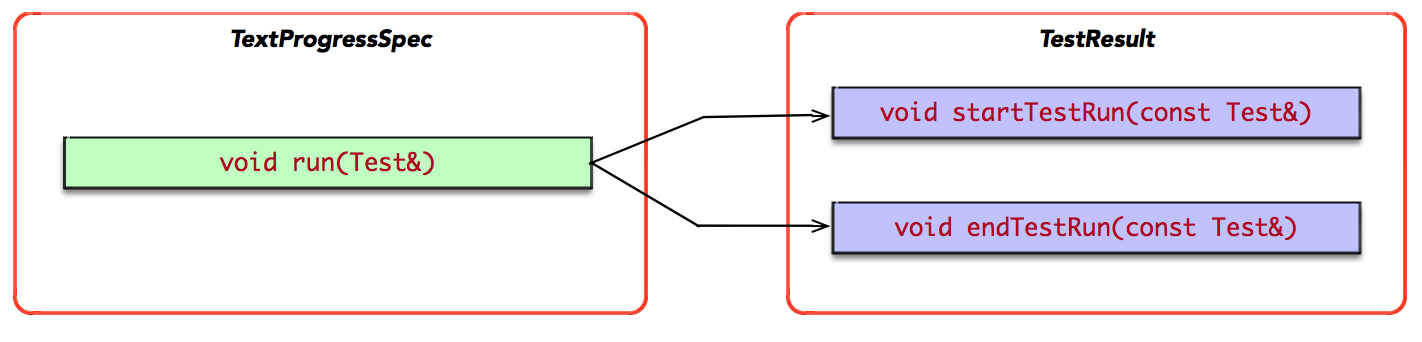
\includegraphics[width=1.0\textwidth]{figures/xunit/coupling-3.png}
\caption{重构之前}
 \label{fig:coupling-3}
\end{figure}

根据迪米特法则,将\ascii{TextProgressSpec::run}搬迁至\ascii{TestResult::runRootTest}。一方面,\ascii{TestResult}暴露给\ascii{TextProgressSpec}的接口由\ascii{2}减少至\ascii{1},缓解了\ascii{TextProgressSpec}对\ascii{TestResult}的依赖关系。另一方面,内联化\ascii{TestResult::startTestRun, TestResult::endTestRun},使得\ascii{TestResult}获得了更好的封装性。

\begin{figure}[H]
\centering
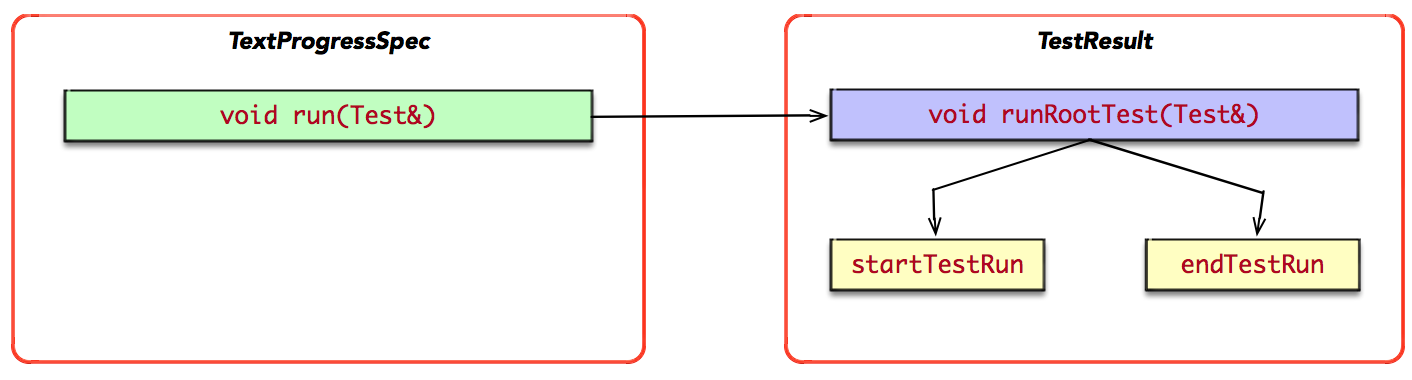
\includegraphics[width=1.0\textwidth]{figures/xunit/decoupling-3.png}
\caption{重构之后}
 \label{fig:decoupling-3.png}
\end{figure}

与之前两个重构手法不一样,此处无需进一步地抽象,例如提取抽象接口\ascii{BareTest},因为\ascii{TestResult}不依赖于\ascii{TextProgressSpec}。简单搬迁\ascii{TextProgressSpec::run}的实现逻辑至\ascii{TestResult::runRootTest}即可。

\begin{figure}[H]
\centering
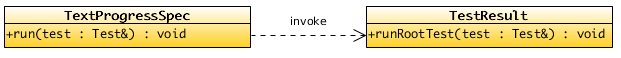
\includegraphics[width=0.8\textwidth]{figures/xunit/bare-test-uml.png}
\caption{搬迁职责:TestResult::runRootTest}
 \label{fig:bare-test-uml}
\end{figure}

\end{content}
